\section{Benchmark}
Um die Performance von Videospielen zu testen, kann man Benchmarking durchführen. Ein Benchmark ist ein Maßstab um Leistungen zu vergleichen. Hier wird das ECS mit dem objektorientierten Spiel (im Folgenden Mono genannt) verglichen. Außerdem ist die Leistungsfähigkeit zwischen ECS und Mono besonders interessant, weshalb in diesem Benchmark die Zeit gemessen wird, die ein Bild zur Berechnung gebraucht hat. Eine andere oft verwendete Einheit ist es die durchschnittlichen Bilder pro Sekunde anzugeben (fps). Die Umrechnung ist hierbei wiefolgt: $1 fps = \frac{1}{1 ms * 0.001} $\\
In diesem Kapitel wird nun der direkte Vergleich von ECS und Mono angestellt. Dazu stellt Unity einige hilfreiche Tools zu Verfügung um Aspekte in einem Spiel zu messen. Auch können man dadurch gut nachvollziehen, wie lange eine Aufgabe, wie zum Beispiel die Ausführung der Update Funktionen, benötigt hat. Bei den nachfolgenden Tests wird jeweils das implementierte Spiel, welches in \hyperref[sec:factory]{Kapitel \ref*{sec:factory}} vorgestellt wurde, verwendet. Es werden immer 2000 Bilder gemessen, wobei die letzten 2000 Bilder aufgezeichnet werden, sobald ein Stahlbarren hinten in dem Kasten angekommen ist (\hyperref[fig:steel]{Abbildung \ref*{fig:steel}}). Zusätzlich werden mehrere Durchläufe gemacht. Angefangen wird mit einer, 10 und 100 Fabriken. In 100er Schritten werden dann die Fabriken erhöht, bis zu 1000 Fabriken.\\
Um die Benchmark Tests reproduzierbar zu machen gibt es zunächst eine Auflistung der Komponenten, auf denen die Tests durchgeführt wurden: NVIDIA GeForce RTX 3070, Intel Core i7 12700, 32 Gb DDR 4 RAM. Die Tests liefen außerdem auf einem Windows 11 Betriebssystem.
\subsection{Profiler}
Der Unity Profiler ist ein Tool, mit dem man Performance Informationen über sein Spiel bekommt. Mit dem Profiler kann man sein Spiel aufzeichnen und Daten über eine festgelegte Anzahl von Bildern sammeln. Dazu gehören die CPU Auslastung, der Speicherverbrauch, wie viele Objekte gezeichnet werden und noch vieles mehr. Während das Spiel ausgeführt wird gibt werden diese Daten live gezeigt. Zusätzlich lassen sich die Daten auch beim Pausieren des Spiel abspeichern und andere gespeicherte Daten wieder laden um sie zu betrachten. \hyperref[fig:profiler]{Abbildung \ref*{fig:profiler}} zeigt den Profiler und schon aufgezeichnete Daten. 
\begin{figure}[H]
\centering
\begin{annotatedFigure}
	{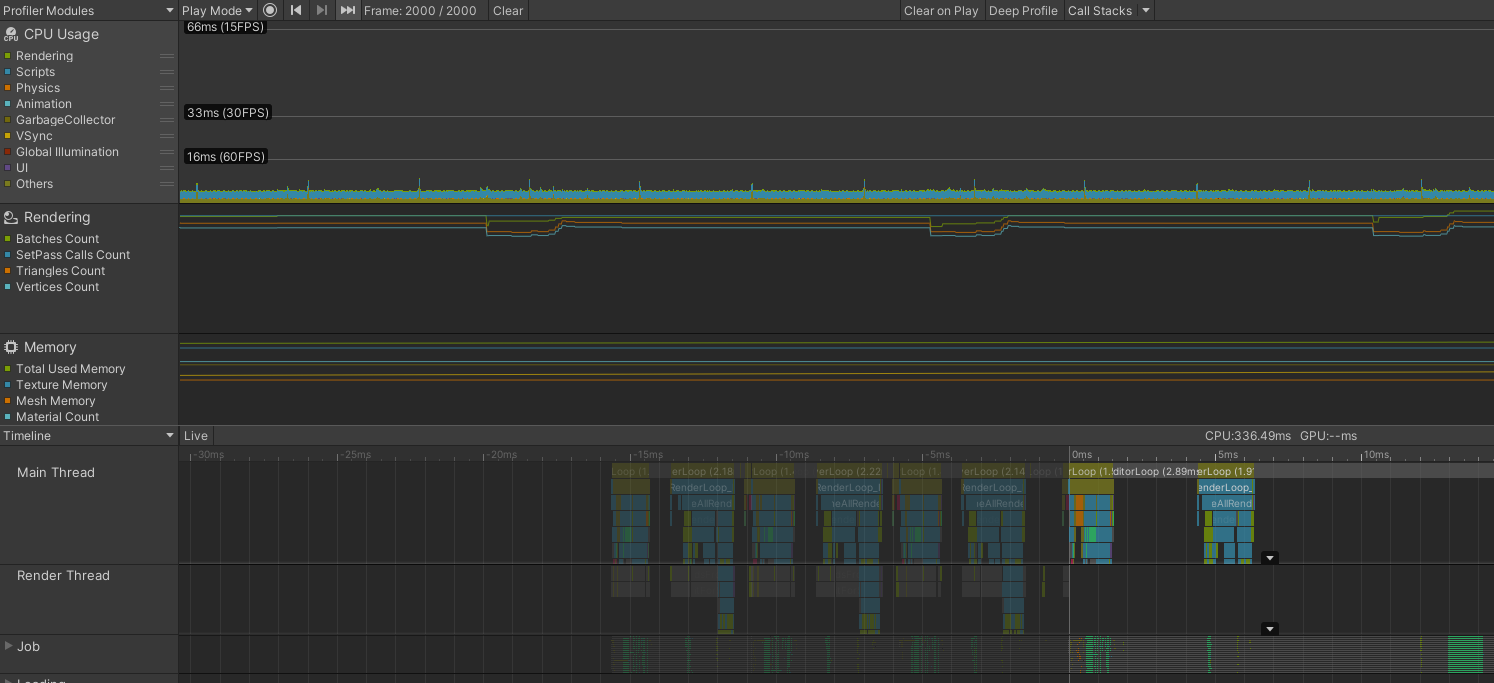
\includegraphics[scale=0.428]{Bilder/Profiler.png}}
    \annotatedFigureBox{0.1688,0.9496}{0.363,1.01}{A}{0.363,0.9496}
	\annotatedFigureBox{0.12,0.65}{1.005,0.76}{B}{1.005,0.65}
	\annotatedFigureBox{-0.005,0.3778}{0.1259,1.01}{C}{0.1259,0.3778}
	\annotatedFigureBox{0.38,0.0888}{0.8705,0.3831}{D}{0.8705,0.0888}
\end{annotatedFigure}
\caption{Der Profiler in dem Unity Editor. Mit ihm lässt sich die Auslastung des Spiels während dem Spielen aufzeichnen und die Daten zur weiteren Verwendung abspeichern. In der oberen Leiste (A), lässt sich das Spiel wie gewünscht aufzeichnen und man sieht die Anzahl an aufgezeichneten Bildern. Man kann auch einzelne Bilder auswählen. Darunter (B) sieht man den Verlauf der aufgezeichneten Bilder. Hier sieht man für jedes Modul eine Auslastung über den Verlauf der 2000 Bildern. Links (C) kann man die einzelnen Module sehen. Sichtbar sind hier die Module CPU Usage, Rendering und Memory, wobei man für weitere im Editor nach unten scrollen muss. Unten (D) ist eine genauere Timeline sichtbar, da hier nur einige Bilder abgebildet werden.}
\label{fig:profiler}
\end{figure}
In der \hyperref[fig:profiler]{Abbildung \ref*{fig:profiler}} erkennt man die einzelnen Auslastungen und ihre Kategorien. Zusätzlich kann man ein bestimmtes Bild auswählen und erhält dazu weitere Details in der Timeline weiter unten. Diese aufgezeichneten Daten lassen sich dann in dem Profile Analyzer weiter analysieren.
\subsection{Profile Analyzer}
Der Profile Analyzer dient der weiteren Analyse von aufgenommenen Profilen mit dem Profiler. Zusätzlich hat man mit dem Profile Analyzer die Möglichkeit zwei Profile direkt miteinander zu vergleichen. Dies zeigt \hyperref[fig:profile_analyzer]{Abbildung \ref*{fig:profile_analyzer}}.
\begin{figure}[H]
\centering
\begin{annotatedFigure}
	{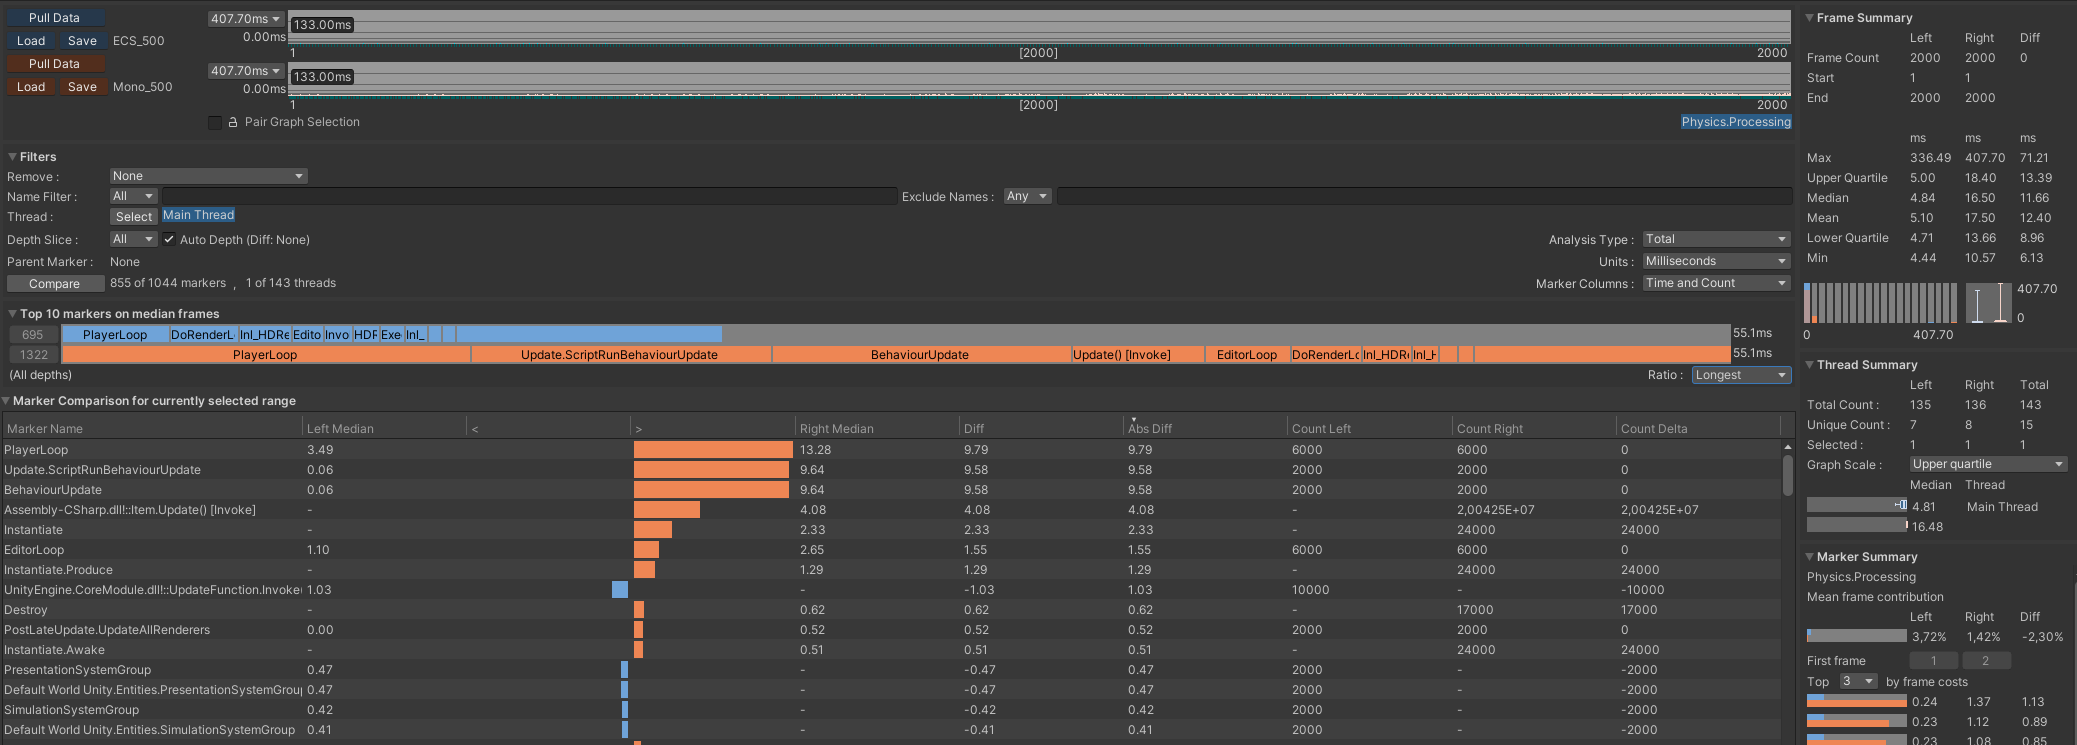
\includegraphics[scale=0.31]{Bilder/Profile Analyzer.png}}
	\annotatedFigureBox{-0.005,0.8046}{0.182,1.01}{A}{0.182,0.8046}
	\annotatedFigureBox{0.86,-0.01}{1.005,1.01}{D}{1.005,-0.01}
	\annotatedFigureBox{-0.005,0.4842}{0.857,0.5942}{B}{0.857,0.4842}
	\annotatedFigureBox{-0.005,-0.01}{0.445,0.4804}{C}{0.445,-0.01}
\end{annotatedFigure}
\caption[Der \textit{Profile Analyzer} im Unity Editor]{Der \textit{Profile Analyzer} im Unity Editor. Es werden die Mono- und die \textit{ECS} Messdaten des Spiels miteinander verglichen. Links oben (A) erkennt man, welche Daten man gerade vergleicht und sieht dazu eine Timeline beider Daten. Die \textit{ECS} Daten sind im Bild blau dargestellt, die Mono Daten rot. In der Mitte des Bildes (B) hat man den Vergleich des Median Bildes. Deutlich zu erkennen ist die wesentlich kürzere Laufzeit des \textit{ECS} Bildes. In dem unteren Teil (C) werden wichtige Spielfunktionen im Vergleich dargestellt. Beispielsweise ist ganz oben der \textit{PlayerLoop} (gesamte Berechnungszeit eines Bildes). Dazu erkennt man an dem Balken, welches der Spiele eine höhere Berechnungszeit hatte. Rechts (D) gibt es zusätzlich noch eine Zusammenfassung über die gesamte Anzahl an Bildern und Threads in beiden Spielen.}
\label{fig:profile_analyzer}
\end{figure}
Oberhalb erkennt man beide Daten die man vergleichen möchte und wie viele Bilder die beiden Daten enthalten. Hier ist erkennbar, dass einmal die Daten des ECS mit 500 Fabriken (blau dargestellt) und des Mono's mit 500 Fabriken (rot dargestellt) verglichen werden. Die wichtigen Teile sind hierbei die zusammenfassende Übersicht (rechts), welche eine Übersicht über alle Bilder oder Threads bietet, und den Vergleich von Kernfunktionen der Spiele, wie beispielsweise der Update Funktionen und dem Erstellen, oder Zerstören von Objekten. Das Problem hierbei ist jedoch, dass die Kernfunktionen von dem Objektorientierten, anders heißen als die von dem datenorientierten und man sie somit schlecht gegenüberstellen kann. Würde man zwei Objektorientierte Spiele vergleichen, hätten beide einen PlayerLoop und man würde direkt erkennen, welcher länger gebraucht hat. Dennoch kann man die Zusammenfassung der Bilder gut Nutzen und deshalb werden diese im Folgenden ausgewertet.
\subsection{Vergleich}
\begin{figure}[H]
\centering
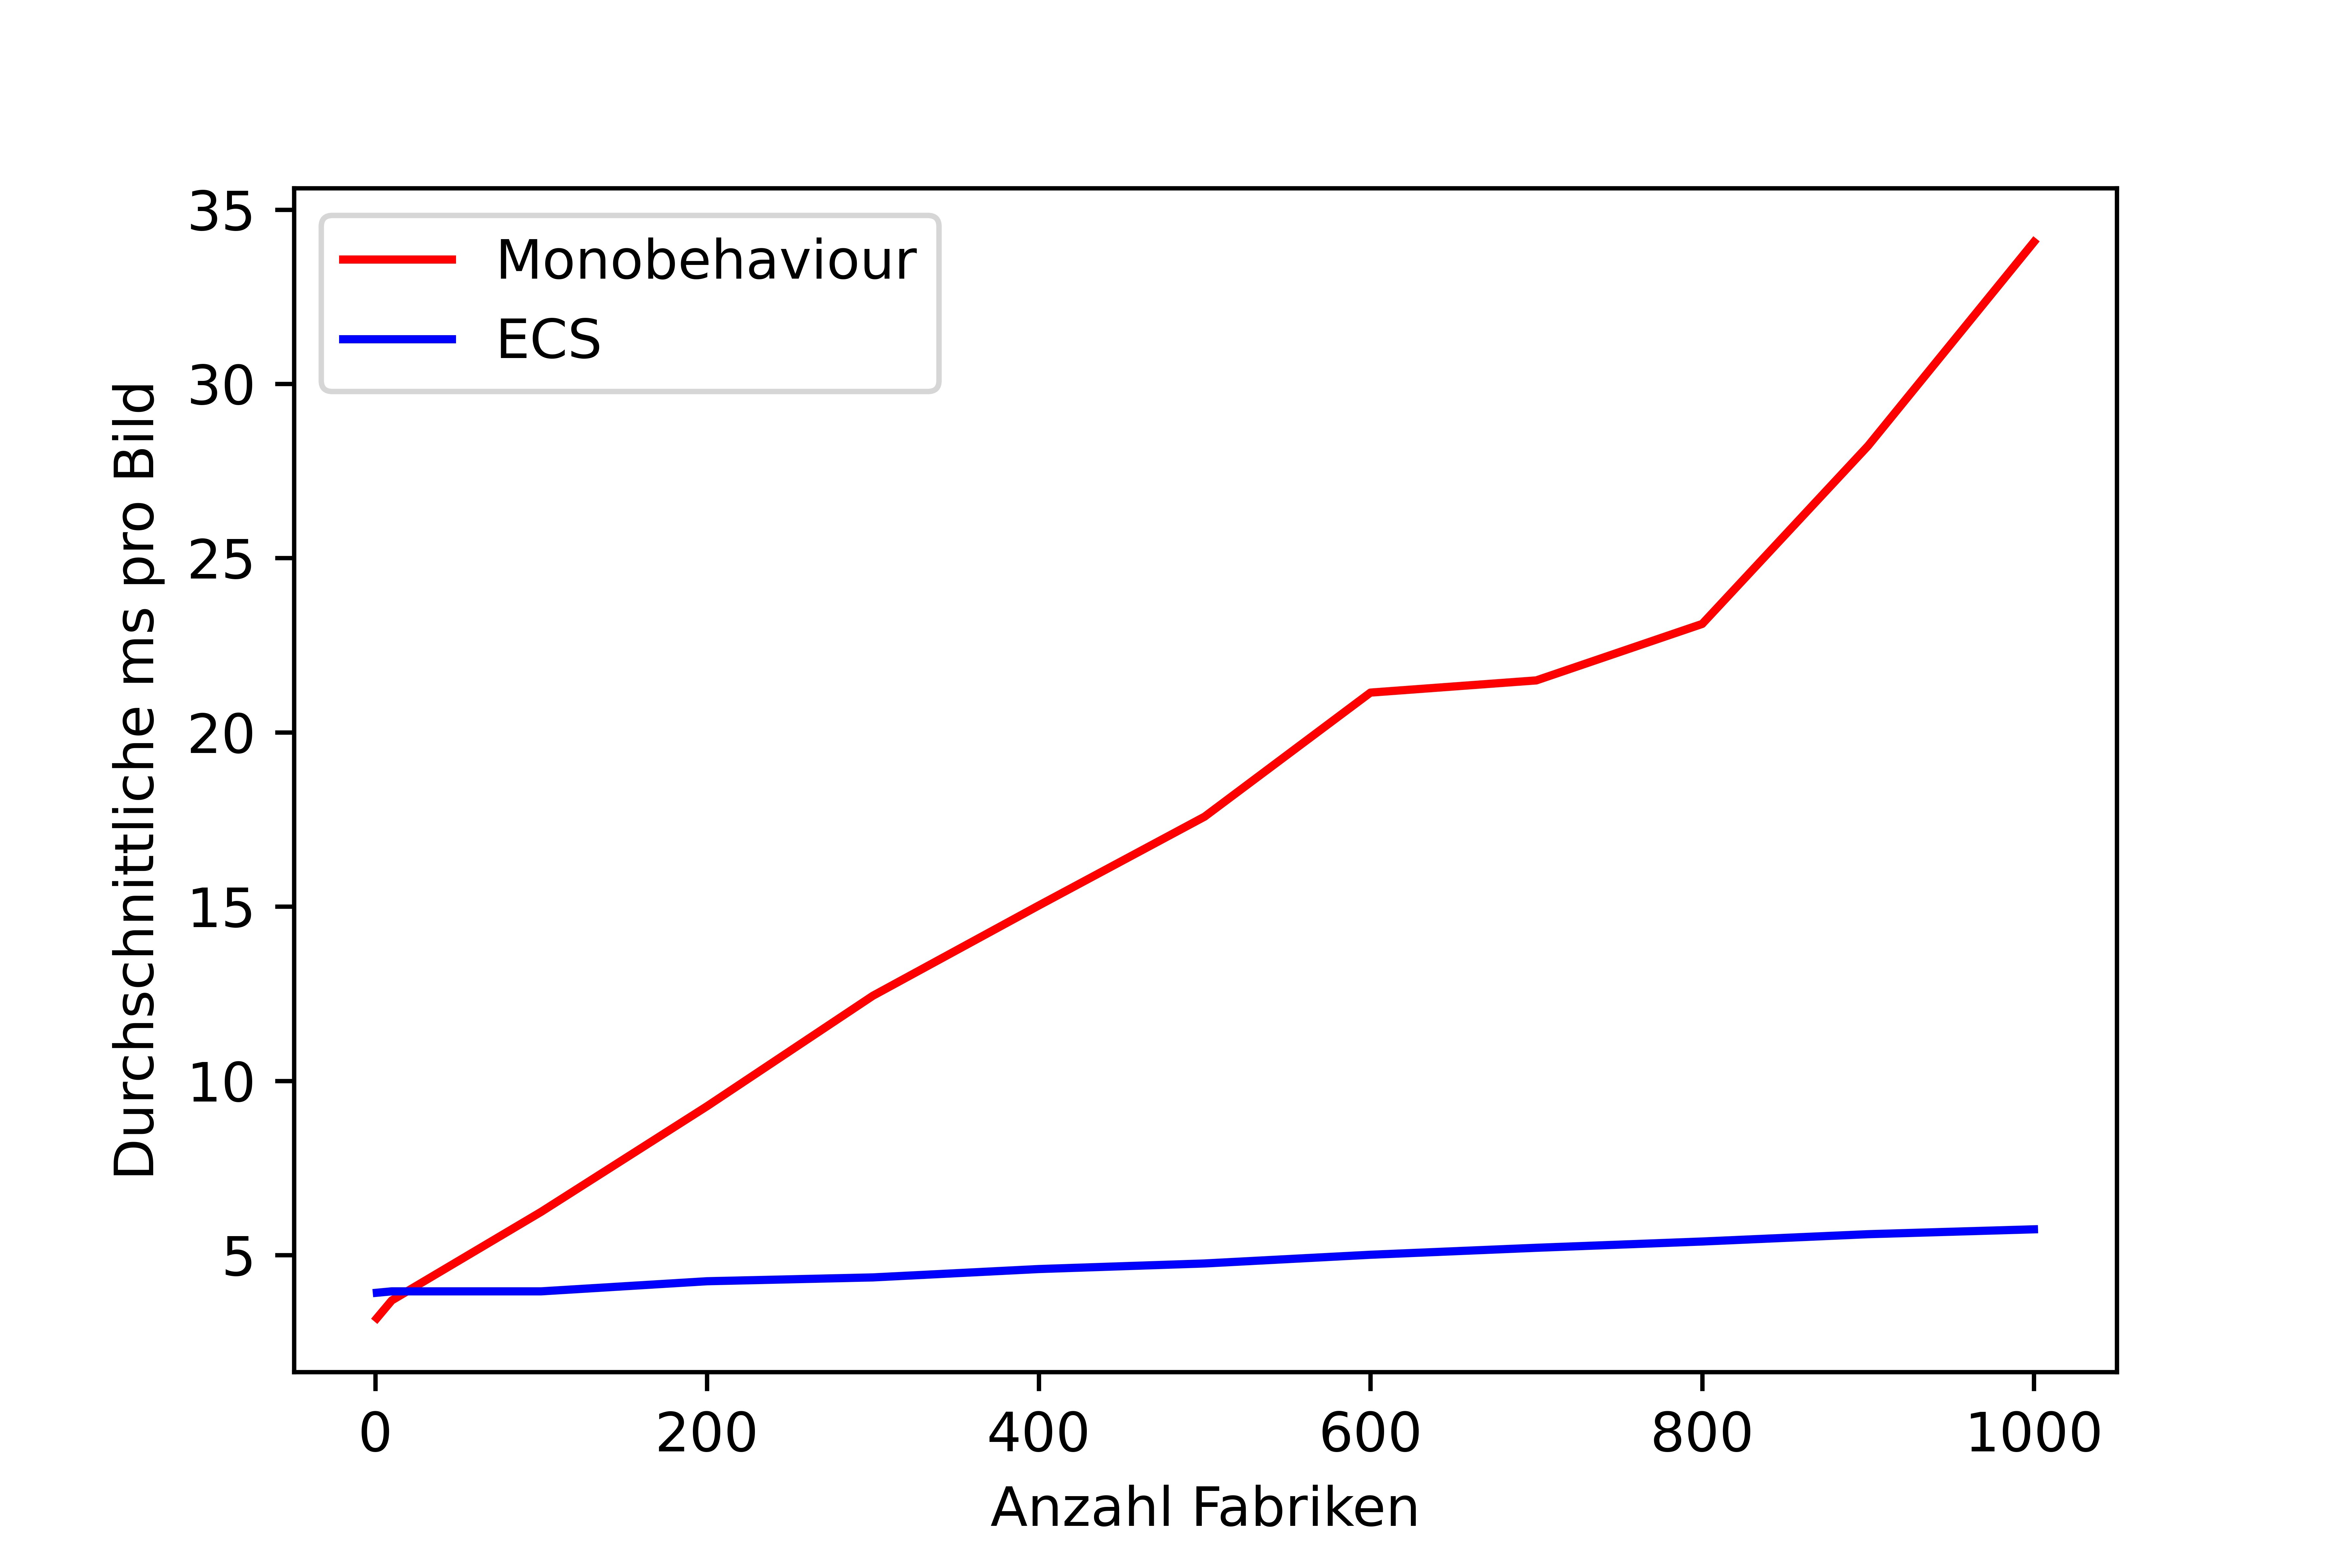
\includegraphics[scale=1]{Bilder/Benchmark.png}
\caption{Der Vergleich von Mono und dem Entity Component System. Es werden die durchschnittlichen Millisekunden, die ein Bild zur Berechnung gebraucht hat, für verschiedene Anzahlen von Fabriken, angezeigt.}
\label{fig:benchmark}
\end{figure}
\begin{tabular}[h]{c|c|c|c|c|c|c}
 & \multicolumn{3}{c|}{ECS} & \multicolumn{3}{c}{Mono}\\
Anzahl Fabriken & Min & Mean & Max & Min & Mean & Max\\
\hline
1 & 2.42 ms & 3.92 ms & 10.94 ms & 2.77 ms & 3.19 ms & 8.65 ms\\
10 & 2.46 ms & 3.96 ms & 10.47 ms & 3.0 ms & 3.7 ms & 9.33 ms\\
100 & 3.57 ms & 3.96 ms & 9.03 ms & 5.27 ms & 6.24 ms & 13.08 ms\\
200 & 2.76 ms & 4.25 ms & 10.87 ms & 7.87 ms & 9.27 ms & 19.16 ms\\
300 & 3.94 ms & 4.36 ms & 9.37 ms & 10.44 ms & 12.44 ms & 25.37 ms\\
400 & 4.18 ms & 4.6 ms & 9.82 ms & 10.61 ms & 15.03 ms & 33.69 ms\\
500 & 4.3 ms & 4.76 ms & 9.81 ms & 11.12 ms & 17.58 ms & 39.04 ms\\
600 & 4.52 ms & 5.01 ms & 10.56 ms & 10.66 ms & 21.14 ms & 61.65 ms\\
700 & 4.48 ms & 5.21 ms & 10.16 ms & 9.33 ms & 21.49 ms & 53.76 ms\\
800 & 4.48 ms & 5.39 ms & 10.89 ms & 8.51 ms & 23.11 ms & 65.15 ms\\
900 & 4.35 ms & 5.6 ms & 10.6 ms & 8.86 ms & 28.22 ms & 76.37 ms\\
1000 & 4.6 ms & 5.74 ms & 10.99 ms & 9.65 ms & 34.07 ms & 90.31 ms\\
\end{tabular}
\\\\
\hyperref[fig:benchmark]{Abbildung \ref*{fig:benchmark}} zeigt den direkten Vergleich der Laufzeiten von Monobehaviour zu dem ECS. Ganz deutlich erkennbar schneidet Mono wesentlich schlechter ab. Mono braucht deutlich länger um ein Bild zu verarbeiten, gerade wenn sich die Anzahl der Fabriken erhöht. Also bestätigt das die Annahme, dass das ECS wesentlich besser darin ist große Mengen an Objekten zu verarbeiten. Auch hier steigt die durchschnittliche Zeit ein Bild zu verarbeiten, jedoch nur sehr gering. Eine Ausnahme bildet hier jedoch eine sehr geringe Anzahl an Fabriken. Vor allem bei einer Fabrik ist Mono schneller als das ECS. Das liegt an dem Overhead den das ECS mit sich bringt. Für eine geringe Anzahl an \textit{Entities} ist es ein großer Overhead Jobs mit unterschiedlichen Threads laufen zu lassen. Hier wäre es schneller statt einem Job die Aktionen direkt auf dem main Thread auszuführen.